\section{Validação de projeto}
\label{sec:validacao}

Ao longo do texto, definiu-se os requisitos e como os atingi-los, porém ainda é
preciso estabelecer como ocorrerá a prova do cumprimento do que foi acordado.
Para isso, nessa seção serão propostos alguns testes que são capazes de validar
o cumprimento dos requisitos. Essa etapa de validação poderia ser executada
somente após o desenvolvimento do protótipo, contudo, quaisquer modificações
de projeto com o protótipo já finalizado acrescentaria em um grande custo de
financeiro e em atraso de projeto. Dessa forma, optou-se pela validação do
protótipo via simulação, o que permite testar o veículo em ambiente subaquático
simulado, sem risco de dano ao veículo e evitando grandes retrabalhos por
modificações no projeto. Nessa seção, será discutido como a simulação deve ser
realizada para validação dos requisitos de projeto, assim como a configuração do
ambiente virtual submarino.

\subsection{Módulos de simulação}
\label{sec:simu-modules}

A simulação fidedigna de um veículo submarino deve contar com a simulação dos
atuadores, sensores e da física de um corpo rígido debaixo d'água. Com o objetivo de obter uma simulação que incluísse todos esses tópicos, algumas soluções de \textit{software} disponíveis serão adotas e algumas desenvolvidas, a especificação de cada uma e justificativa de escolha é o objetivo desta seção.

\subsubsection{Sensores, atuadores e física}

As funções de simular o comportamento de um robô no meio com seus sensores e
atuadores é a tarefa de um simulador de robótica, dessa forma, é necessário se
definir qual deve ser utilizado para a validação deste projeto. A tabela da
Figura \ref{fig:simulators-comparison} mostra as alternativas de simuladores
que possuem funcionalidades essenciais para validação de um robô submarino.
Dentre as cinco alternativas apresentadas na tabela, 3 delas utilizam o simulador Gazebo \cite{gazebo}, que são UWSim ({\it Underwater Simulator}), UUV
({\it Unmanned Underwater Vehicle Simulator}) e USVSim ({\it Unmanned Surface
Vehicle Simulator}). Dentre esses, o USVSim seria o mais completo, pois dispoẽ
de quase todas as funcionalidades apresentadas na Figura \ref{fig:simulators-comparison}.

\begin{figure}[h]
    \label{fig:simulators-comparison}
    \caption{Tabela comparativa de simulatores e suas funcionalidades}
    \centering
    \includegraphics[width=1\textwidth]{images/simulators_comparison.png}
\end{figure}

Contudo, o USVSim é desenvolvido a partir do Gazebo, então seria necessário a
instalação de duas ferramentas, sendo que a Open Robotics, empresa desenvolvedora do Gazebo, lançou o novo simulador que substituirá o Gazebo, o
Ignition. Ademais, o Ignition já apresenta as funcionalidades de robótica
submarina incorporadas, dessa forma, optou-se por utilizar somente o \textit{software} Ignition. Nele é possível se carregar um ambiente submarinho 3D assim como o veículo, sendo possível não somente a visualização, mas também obter dados simulados de sensores, controlar motores e simular a interação do robô com o ambiente ao seu redor.

\subsubsection{Comunicação e sensor de distância acústicos}
Apesar do Ignition possibilitar a simulação dos motores e sensores do veículo, a simulação da comunicação e sensor de distância acústicos é uma funcionalidade que não consta no \textit{software}. Portanto, serão desenvolvidos \textit{plugins} para o \textit{software} que simulam as peculiaridades desse tipo sensores. Os \textit{plugins} devem simular atraso da onda sonora na água, ruído e atenuação.


\subsection{Missões}

As missões são tarefas definidas para validação das funcionalidades do veículo, de forma que ao cumprir cada missão, o projeto fica validade a nível de simulação para o cumprimento dos requisitos de projeto.

\subsubsection{Submersão e emersão controlada}
Essa missão consiste em submergir e emergir o ROV a uma determinada profundidade,
como pode ser visto na Figura \ref{fig:descent-test}. Esse procedimento será executado tanto com controle manual de velocidade, como também com controle automático, no qual o ROV se desloca ao longo de um caminho previamente estabelecido. Além disso, arucos seriam posicionados ao longo de todo o trajeto, para obter uma medição mais precisa de profundidade.

\begin{figure}[h]
	\label{fig:descent-test}
	\caption{Missão de submersão e emersão}
	\centering
	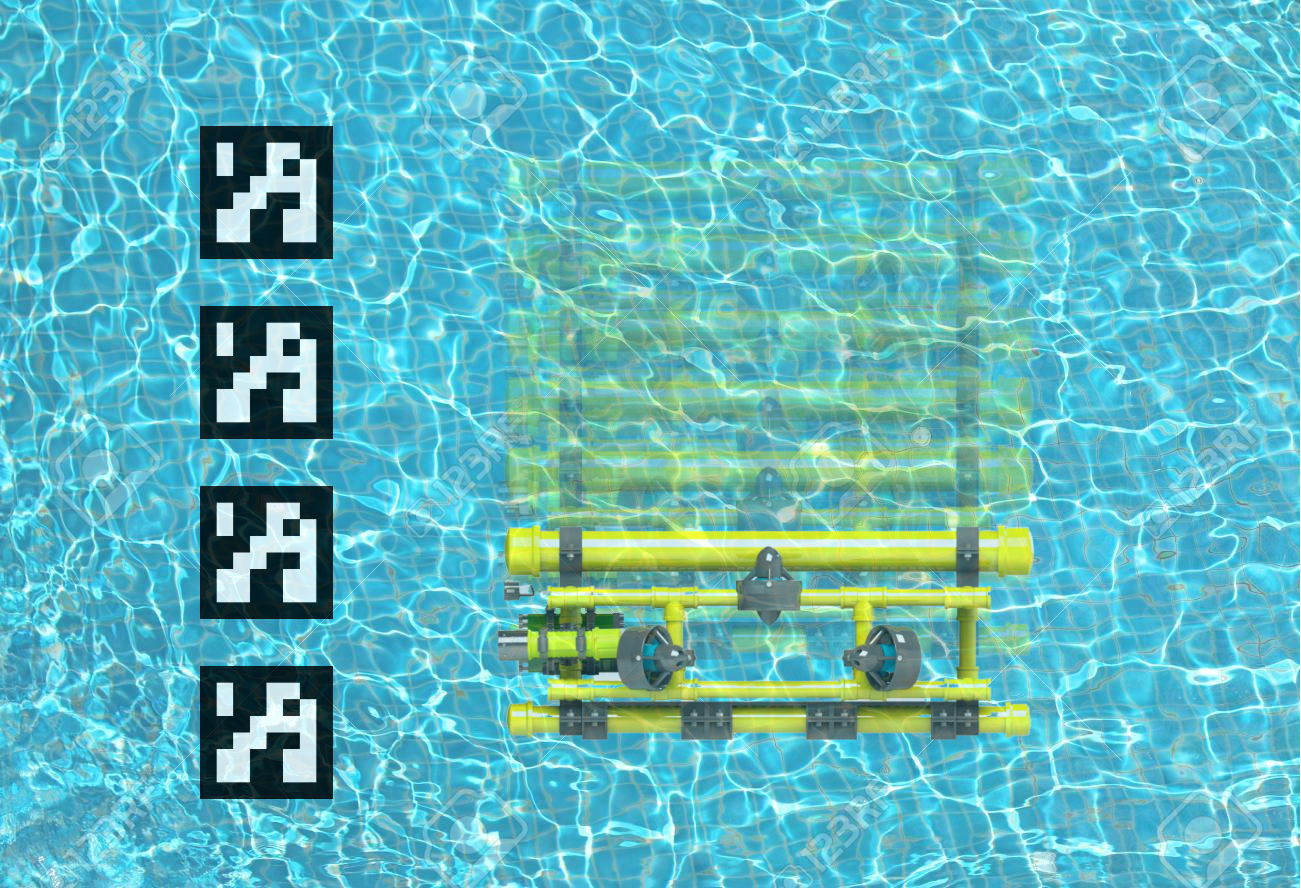
\includegraphics[width=0.8\textwidth]{images/descent_test.png}
\end{figure}

Dessa forma, os requisitos 2, 6 e 7 seriam validados, visto que para a execução dessa tarefa, o ROV deve ser capaz de ir para uma posição previamente conhecida, localizar os arucos e submergir e emergir de forma controlada.

\subsubsection{Teste de velocidade e trajetória circular}

O requisito 3 determina a velocidade máxima que o veículo deve atingir, então é necessário que haja algum teste em que os motores do veículo fiquem no seu máximo para verificar se a velocidade determinada consegue ser atingida. O ROV foi projetado para ter mais velocidade em \textit{surge}, de forma a se deslocar mais rápido ao se mover para frente. Dessa forma, o teste de velocidade consiste em colocar a referência de velocidade no seu valor máximo e medir a velocidade de deslocamento do ROV nesse trecho, porém essa medição é pouco precisa com a configuração de sensores atuais.

Portanto, para medir a velocidade, serão posicionados arucos de diferentes tamanhos e o sistema de SBL. A configuração do ambiente de teste pode ser observada na Figura \ref{fig:speed-test}. Os arucos tem tamanho variado pois quanto maior o aruco, mais longe deve-se estar para medir sua pose com precisão, então arucos de diferentes tamanhos servirão para ter uma boa medição em um intervalo maior de distância do veículo para o aruco.

\begin{figure}[h]
	\label{fig:speed-test}
	\caption{Missão de velocidade máxima e seguimento de trajetória}
	\centering
	\includegraphics[width=0.8\textwidth]{images/speed_test.png}
\end{figure}

Outra missão que será executada nessa mesma configuração é a execução de uma trajetória circular, para validação dos requisitos 4, 6 e 7. Ao se executar a trajetória circular, mantendo a profundidade e mantendo os arucos no campo de visão da câmera, pode-se usar o armazenamento da trajetória para validar se o requisito de seguir uma trajetória realmente foi cumprido.

\subsubsection{Mapeamento de rampa}

A validação do requisito 5, que se refere ao mapeamento do leito marinho, pode ser
validado ao se utilizar um terreno conhecido. Então, propõe-se aqui a execução do simples mapeamento de uma rampa, caso a inclinação da rampa seja semelhante ao do mapeamento, pode-se afirmar que o sistema funciona. O mapeamento não será muito detalhado, visto que irá se adquirir somente informação de 4 pontos, medidos com sensores de distância ultrassom abaixo do ROV. Portanto um cenário simples como uma rampa é adequado para validação. Além disso, também se necessita do aruco para posicionamento do ROV, como na Figura \ref{fig:mapping-test}.

\begin{figure}[h]
	\label{fig:mapping-test}
	\caption{Missão de mapeamento}
	\centering
	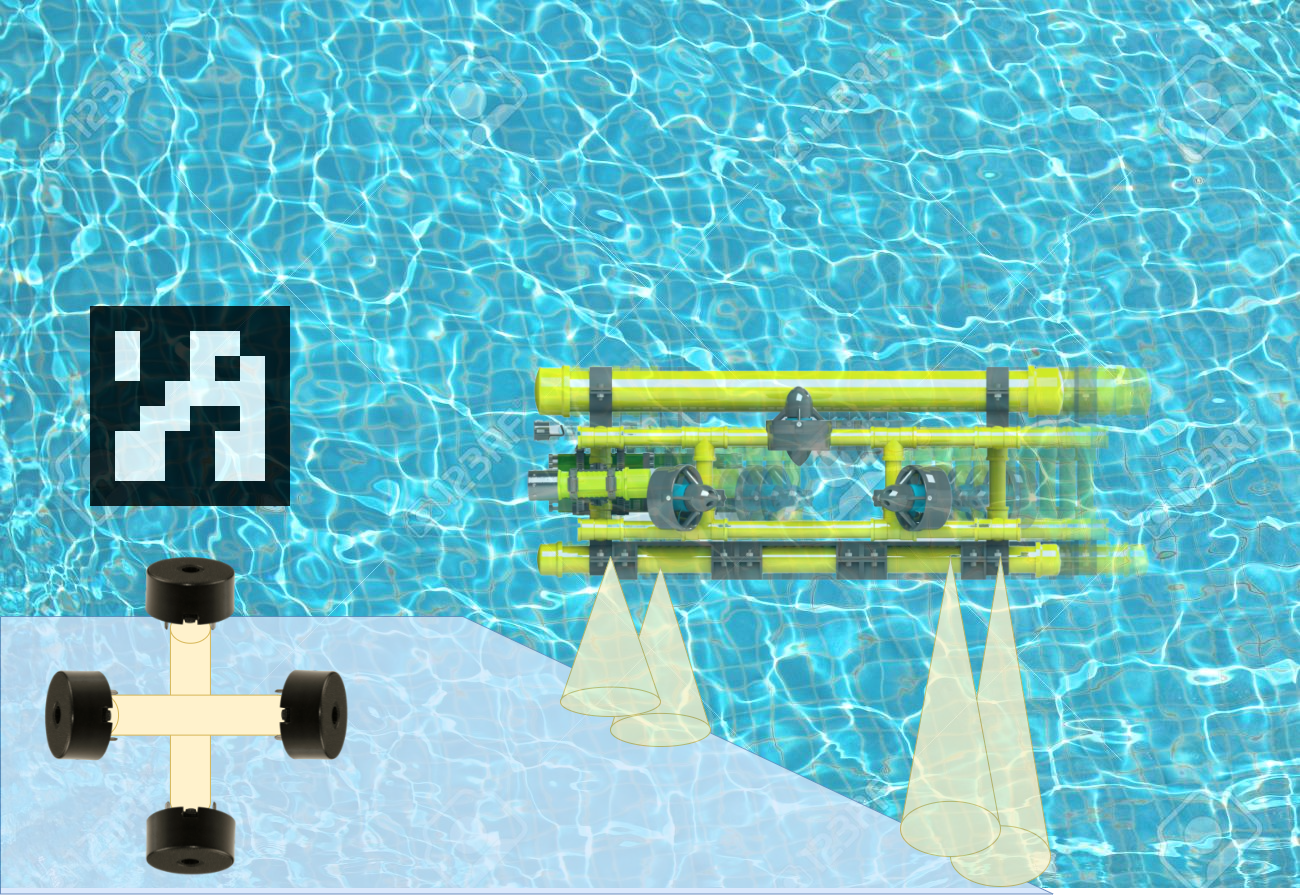
\includegraphics[width=0.8\textwidth]{images/mapping_test.png}
\end{figure}

\subsubsection{Resgate da Moeda}
As missões apresentadas até agora cobriram a validação de todos os requisitos de sistemas que não envolvem resistência e confiabilidade, a validação que está faltando quanto a funcionalidade é a 8. Esse requisito determina que o ROV deve ser capaz de atender um pedido de socorro. Para a validação desse requisito, o BROV deve localizar a caixa de resgate, representada pelo aruco mais à esquerda da Figura \ref{fig:object-retrieving-test}. Além disso, deve esperar o led presente na caixa ascender, a partir daí, o ROV deve se aproximar e capturar a moeda com seu imã e retornar a superfície. Esse teste não só valida o requisito 8, mas como todos os citados anteriormente, a ideia é testar o sistema atendendo todos os requisitos funcionais do ROV ao mesmo tempo. Para esse teste, tanto a localização por aruco como a por SBL .

\begin{figure}[h]
	\label{fig:object-retrieving-test}
	\caption{Tabela comparativa de simulators e suas funcionalidades}
	\centering
	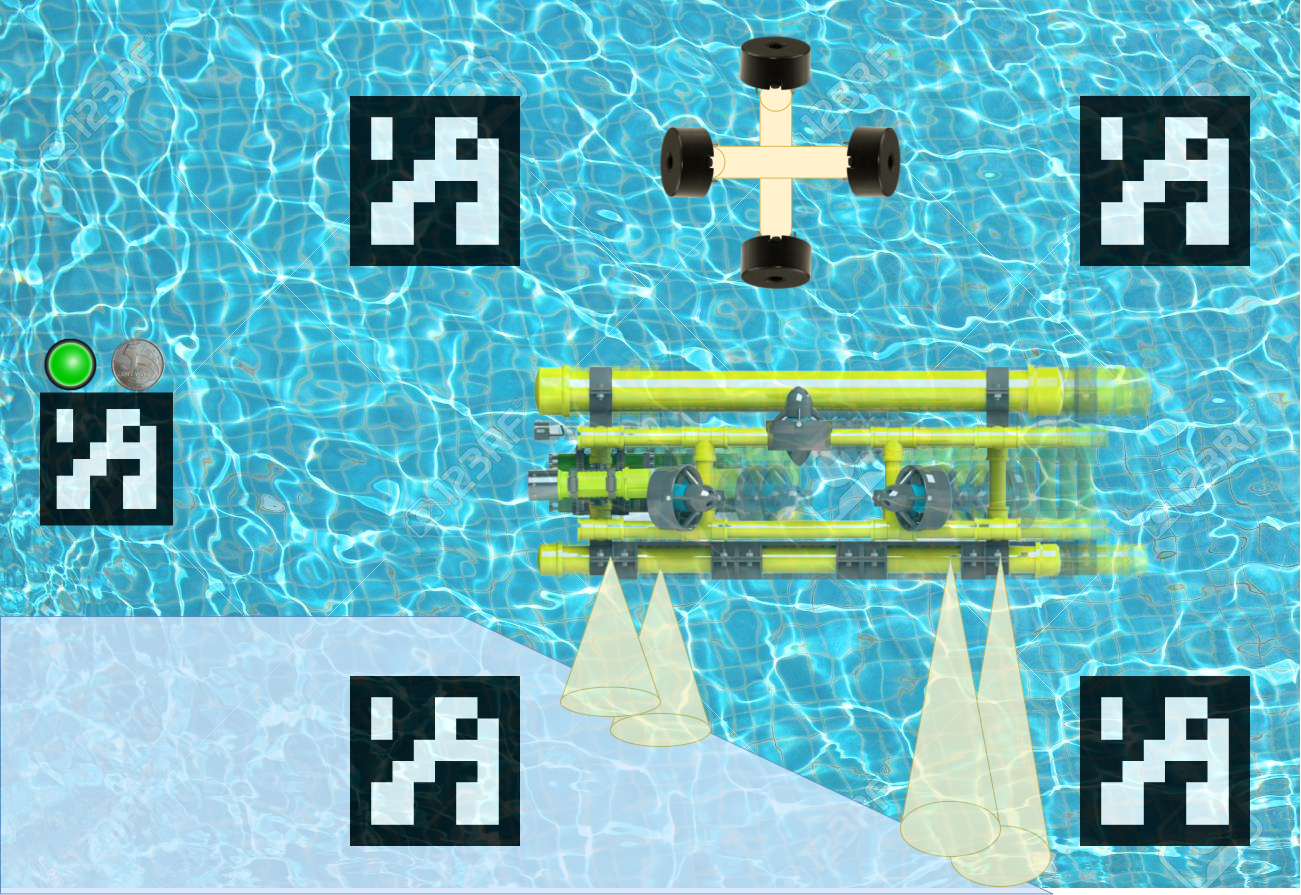
\includegraphics[width=0.5\textwidth]{images/object_retrieving_test.png}
\end{figure}


